\documentclass[10pt, compress]{beamer}

\usetheme{m}

\usepackage{booktabs}
\usepackage[scale=2]{ccicons}
\usepackage{minted}
\usepackage{tikz}
\usepackage[ruled,vlined,english]{algorithm2e}
\usetikzlibrary{arrows,automata,shapes,positioning,calc}

\usepackage{float} % placement des figures
\usepackage{amssymb} % symboles mathématiques
\usepackage{textcomp} % flèche,  intervalle
\usepackage{stmaryrd} % intervalle entiers
\usepackage{graphicx} % affichage d'images
\usepackage{url} % inclure des urls

\newcommand{\first}{\texttt{First}}
\newcommand{\last}{\texttt{Last}}
\newcommand{\sort}{\texttt{Sort}}
\newcommand{\triple}{\texttt{Triple}}
\newcommand{\produ}{\texttt{Normalize}}

\newenvironment{exemple}
{\begin{exampleblock}{Exemple}}
{\end{exampleblock}}

\newenvironment{defi}
{\begin{block}{Définition}}
{\end{block}}

\newcommand{\N}[1]{\left\|#1\right\|_2}


\usepgfplotslibrary{dateplot}

\usemintedstyle{trac}

\title{Projet Pensées Profondes}
\subtitle{}
\date{December 18, 2014}
\institute{École Normale Supérieure de Lyon}

\begin{document}

\maketitle

\begin{frame}[fragile]
Raphaël \textsc{Charrondière}

Marc \textsc{Chevalier}

Quentin \textsc{Cormier}

Tom \textsc{Cornebize}

Yassine \textsc{Hamoudi}

Valentin \textsc{Lorentz}

Thomas \textsc{Pellissier} \textsc{Tanon}

\alert{Adviser:} Eddy \textsc{Caron}
\end{frame}

The {\em Projet Pensées Profondes} (Deep Thought Project) aims at
providing a powerful software for answering questions written in
natural language.
To accomplish this, we developped an eponymous set of tools that
accomplish different tasks and fit together thanks to a protocol
we developped.

These various tasks include data querying (using the young and open
knownledge base Wikidata), question parsing (using the
CoreNLP software written by Stanford University and machine learning),
requests routing, web user interface, and feedback reporting.

Given the young age of this projet, these pieces are only starting
to emerge with their first features and mutual communications,
so we will describe them separately in this document without
much of a general overview of the project.


\section{Overview}
\begin{frame}[fragile]
    \frametitle{Architecture}
    \begin{figure}
        \resizebox{.9\linewidth}{!}{
            \newlength{\moduledistance}
\setlength{\moduledistance}{1cm}
\overfullrule=2cm
\tikzset{
    module/.style={
           rectangle,
%           rounded corners,
           draw=mDarkTeal, very thick,
           minimum width=3cm,
           minimum height = 0.7cm,
           node distance = 1.5cm,
           inner sep=2pt,
           text centered,
           },
}

\tikzset{
    core/.style={
           circle,
           draw=mDarkTeal, very thick,
           minimum width=2cm,
           inner sep=2pt,
           text centered,
           },
}

\tikzset{
    arrow/.style={
           ->,
           draw=mDarkTeal, very thick,
    }
}

\tikzset{
    darrow/.style={
           <->,
           draw=mDarkTeal, very thick,
    }
}

\begin{tikzpicture}[->,>=stealth']
    \node[core] (core) {
        Core
    };
    \node[module,
          right of=core,
          right=\moduledistance,
          ] (grammatical) {
          Grammatical
    };
    \node[module,
          below of=grammatical,
          ] (standalone) {
        \begin{tabular}{c}
        Machine Learning\\Standalone
        \end{tabular}
    };
    \node[module,
          above of=grammatical,
          ] (reformulation) {
        \begin{tabular}{c}
        Machine Learning\\Reformulation
        \end{tabular}
    };
    \node[module,
          left of=core,
          left=\moduledistance,
          ] (wikidata) {
        Wikidata
    };
    \node[module,
          above of=wikidata,
          ] (cas) {
        Computer Algebra
    };
    \node[module,
          below of=wikidata,
          ] (spellchecker) {
        Spell-checker
    };
    \node[module,
          above of=core,
          above=1cm,
          ] (webui) {
        \begin{tabular}{c}
        Web User\\
        Interface
        \end{tabular}
    };
    \node[module,
          above of=reformulation,
%          right=\moduledistance,
          ] (logging) {
        Logging backend
    };
    \draw[mLightBrown,thick] ($(reformulation.north west)+(-0.3,0.3)$)  rectangle node[yshift=-2.5cm,below] {Question Parsing} ($(standalone.south east)+(0.3,-0.3)$);
    \draw[mLightBrown,thick] ($(cas.north west)+(-0.3,0.3)$)  rectangle node[yshift=-2.5cm,below] {Other modules} ($(spellchecker.south east)+(0.3,-0.3)$);

    \draw [darrow] (core)          -- node{} (cas.south east);
    \draw [darrow] (core)          -- node{} (wikidata.east);
    \draw [darrow] (core)          -- node{} (spellchecker.north east);
    \draw [darrow] (core)          -- node{} (reformulation.south west);
    \draw [darrow] (core)          -- node{} (grammatical.west);
    \draw [darrow] (core)          -- node{} (standalone.north west);
    \draw [darrow] (core)          -- node{} (webui.south);
    \draw [darrow] (webui)         -- node{} (logging.west);
    \draw [arrow]  (logging)       -- node{} (reformulation.north);
    \draw [arrow]  (grammatical)   -- node{} (reformulation.south);

\end{tikzpicture}

        }
    \end{figure}
\end{frame}

\begin{frame}[fragile]
    \frametitle{Datamodel}
    How to represent formally a question asked in natural language?

    \alert{Tree} structure.
\end{frame}
\begin{frame}[fragile]
    \frametitle{Datamodel \--- Leaves: resources}
        \begin{itemize}
            \item Strings: "Isaac \textsc{Newton}"
            \item Dates: 25 December 1642
            \item Geographic coordinates: 47° 30' 18'' N ; 9° 44' 57'' E
            \item \ldots
        \end{itemize}
\end{frame}
\begin{frame}[fragile]
    \frametitle{Datamodel \--- Nodes: operations}
        \begin{itemize}
            \item Full \alert{triples}: (Isaac \textsc{Newton}, birth date, 25 December 1642 (Julian)) $\rightarrow$ true
            \item Missing: (?, birth date, 25 December 1642 (Julian)) $\rightarrow$ [Isaac \textsc{Newton}]
            \item Union, Intersection, Difference, \ldots
            \item And, Or, Not
            \item Exists
            \item Sort, First, Last
        \end{itemize}
\end{frame}

\begin{frame}[fragile]
    \frametitle{Datamodel \--- Examples}
    \begin{itemize}
        \only<1>{
        \item \alert{"Is Brussels the capital of Belgium and the European Union?"}
          \begin{center}
            \begin{figure}
          \resizebox{\linewidth}{!}{
            \begin{tikzpicture}
              \node (0) at (10,8.5) {$\bigwedge$};
              \node (1) at (7,7) {$\triple$};
              \node (11) at (5,5.5) {Brussels};
              \node (12) at (7,5.5) {capital};
              \node (13) at (9,5.5) {Belgium};
              
              \node (2) at (13,7) {$\triple$};
              \node (21) at (11,5.5) {Brussels};
              \node (22) at (13,5.5) {capital};
              \node (23) at (15,5.5) {European Union};

              \node (9) at (14,1) {}; % utilisé pour forcer le positionnement de la figure globale

              \draw[->, >=latex] (0) edge node[sloped, anchor=center, above] {} (1);
              \draw[->, >=latex] (1) edge node[sloped, anchor=center, above] {\scriptsize{subj.}} (11);
              \draw[->, >=latex] (1) edge node[sloped, anchor=center, above] {\scriptsize{pred.}} (12);
              \draw[->, >=latex] (1) edge node[sloped, anchor=center, above] {\scriptsize{obj.}} (13);
              \draw[->, >=latex] (0) edge node[sloped, anchor=center, above] {} (2);
              \draw[->, >=latex] (2) edge node[sloped, anchor=center, above] {\scriptsize{subj.}} (21);
              \draw[->, >=latex] (2) edge node[sloped, anchor=center, above] {\scriptsize{pred.}} (22);
              \draw[->, >=latex] (2) edge node[sloped, anchor=center, above] {\scriptsize{obj.}} (23);
             \end{tikzpicture}
            }
            \end{figure}

          \end{center}}
            
        \only<2>{
        \item \alert{"Who is the mayor of the capital of Kreis Bergstraße?"}
          \begin{center}
            \begin{forest}
              [\texttt{Triple}[\texttt{Triple}[Kreis Bergstraße][capital][?]][mayor][?]]
            \end{forest}
          \end{center}}
            
        \only<3>{
          \item \alert{"What is the birth date of the first president of Germany?"}
          \begin{center}
            \begin{forest}
              [\texttt{Triple}[\texttt{First}[\texttt{Sort}[\texttt{Triple}[Germany][president][?]][mandate begin date]]][birth date][?]]
            \end{forest}
          \end{center}}

        \only<4>{
          \item \alert{"Is there a medical treatment for Ebola?"}
            \begin{center}
              \begin{forest}
                [\texttt{Exists}[\texttt{Triple}[Ebola][medical treatment][?]]]
              \end{forest}
            \end{center}}

        \only<5>{
          \item \alert{"Who are the children of François \textsc{Mitterrand} and Anne \textsc{Pingeot}?"}
            \begin{center}
              \begin{forest}
                [$\bigcap$[\texttt{Triple}[François \textsc{Mitterrand}][child][?]][\texttt{Triple}[Anne \textsc{Pingeot}][child][?]]]
              \end{forest}
            \end{center}}


    \end{itemize}
\end{frame}


\section{Question parsing}


\begin{frame}[fragile]

Map the input question to the most relevant normal form.
  
\onslide<2->{
\begin{center}
  \alert{Where does the prime minister of United Kingdom live?}
\end{center}}

\begin{figure}
 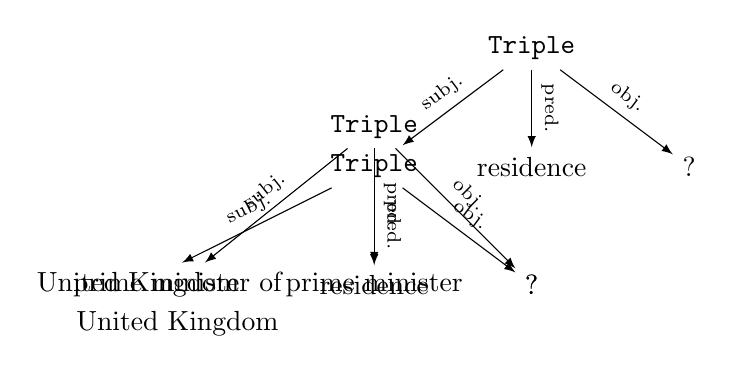
\begin{tikzpicture}
  \onslide<2>{
  \node (7) at (8,9) {$\triple$};
  \node (8) at (5.5,7) {prime minister of};
  \node (11) at (5.5,6.5) {United Kingdom};
  \node (9) at (8,7) {residence};
  \node (10) at (10,7) {?};

  \draw[->, >=latex] (7) edge node[sloped, anchor=center, above] {\scriptsize{subj.}} (8);
  \draw[->, >=latex] (7) edge node[sloped, anchor=center, above] {\scriptsize{pred.}} (9);
  \draw[->, >=latex] (7) edge node[sloped, anchor=center, above] {\scriptsize{obj.}} (10);}
  
  \onslide<3>{  
  \node (0) at (10,10) {$\triple$};
  \node (1) at (10,8.5) {residence};
  \node (2) at (12,8.5) {?};
  \node (3) at (8,8.5) {$\triple$};
  \node (4) at (8,7) {prime minister};
  \node (5) at (5,7) {United Kingdom};
  \node (6) at (10,7) {?};

  \draw[->, >=latex] (0) edge node[sloped, anchor=center, above] {\scriptsize{obj.}} (2);
  \draw[->, >=latex] (0) edge node[sloped, anchor=center, above] {\scriptsize{pred.}} (1);
  \draw[->, >=latex] (0) edge node[sloped, anchor=center, above] {\scriptsize{subj.}} (3);
  \draw[->, >=latex] (3) edge node[sloped, anchor=center, above] {\scriptsize{subj.}} (5);
  \draw[->, >=latex] (3) edge node[sloped, anchor=center, above] {\scriptsize{obj.}} (6);
  \draw[->, >=latex] (3) edge node[sloped, anchor=center, above] {\scriptsize{pred.}} (4);}
 \end{tikzpicture}
\end{figure}

\end{frame}


\section{Grammatical approach}

Trees of triples can be produced after analysing the grammatical structure of sentences. First, we  present the tool we use to extract grammatical dependencies. Then, we expose chronologically our algorithm to product triples from grammatical structure.

We will detail throughout this section our algorithm on the example:
\begin{center}
 \textit{What is the birth date of the president of the United States?}
\end{center}

%########################################################################################%

\subsection{\Stanford}

The \Stanford library \footnote{\url{http://nlp.stanford.edu/software/corenlp.shtml}} is a tool developed by the \emph{Stanford Natural Language Processing group}, composed of linguists and computer scientists. This software is well-documented and considered as a ``state of the art'' tool. Moreover, it includes very efficient grammatical parsers.

Since this library is written in Java, and our module in Python, we use a Python wrapper\footnote{\url{https://bitbucket.org/ProgVal/corenlp-python/overview}} we first patched to support Python 3 and some features the wrapper did not implement.

We use \CoreNLP mostly to get grammatical dependency trees from input questions. It consists in trees which nodes are the words of the sentence, and edges reflect the grammatical relations between words.

Figure \ref{tree_one} provides an overview of such a tree on our question example \emph{What is the birth date of the president of the United States?}. For instance, the edge:
  \[\texttt{president}\xrightarrow{\texttt{det}}\texttt{the}\]
means that \emph{the} is a determiner for \emph{president}.

\begin{figure}
  \centering
  \caption{Dependency tree}
  \label{tree_one}
    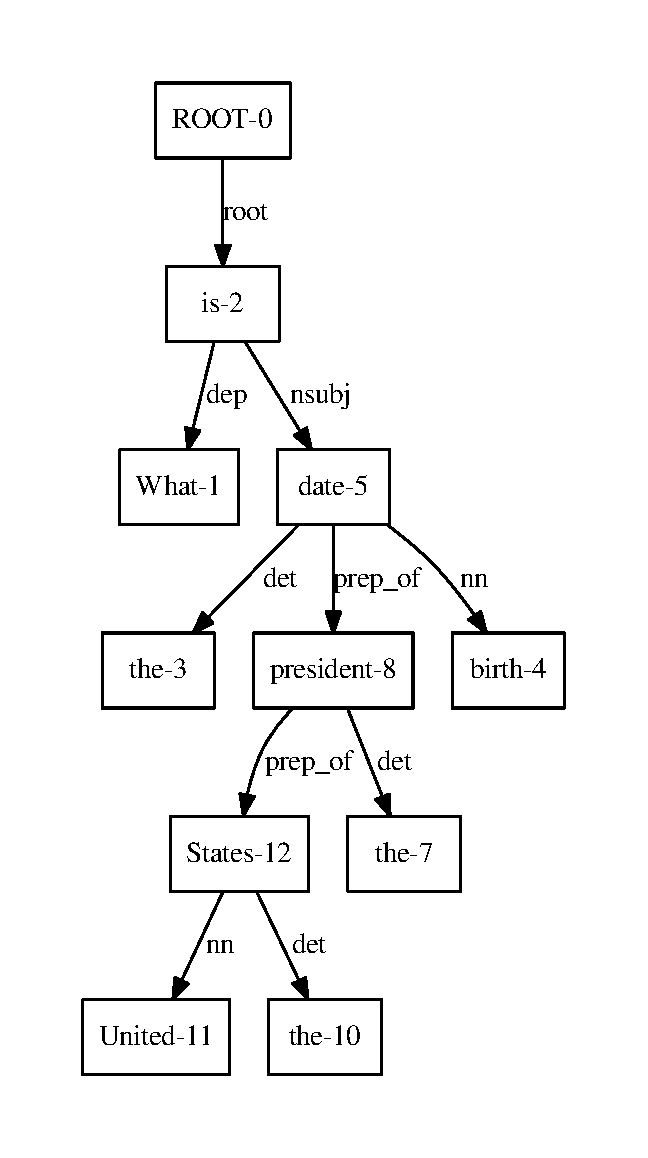
\includegraphics[scale=0.6]{../examples_NLP_grammatical/tree1.pdf}
\end{figure}

Some nodes of this tree are also endowed with tags. For example, \emph{United} and \emph{States} have the tag \emph{location}.

The Stanford typed dependencies manual (\cite{stanfordDep}) provides a full list and description of possible grammatical dependencies.

%########################################################################################%

\subsection{Preprocessing}

The preprocessing consists in a sequence of operations executed on the tree outputs by the \Stanford library. The aim is to simplify it, by merging the nodes which should belong together.

The current version of the module performs two sorts of merges:
\begin{itemize}
    \item \textbf{Merge quotation nodes.} This operation merges all the nodes which are in a same quotation (delimited by quotation marks). It also adds the words
    of the quotation which were deleted by the \Stanford library (e.g. \emph{in}, \emph{of}\dots). The final result is a node, containing the
    exact quotation, and placed at the appropriate position in the tree.
    
    \item \textbf{Merge named entities.} The \Stanford library performs a \emph{named entities recognition} (NER), which provides informative 
    tags in some nodes. For instance, \emph{United} and \emph{States} are tagged \emph{LOCATION} (see figure \ref{tree_two}). In the preprocessing step, we merge all neighbour nodes with a same NER tag. In our example, we merge the two nodes \emph{United States} into one single node.
\end{itemize}

The preprocessing also identifies the question word (Who, What, Where...) and removes it from the dependency tree.

Preprocessing is illustrated on figure \ref{tree_two}. The question word is \textit{What}.

\begin{figure}
  \centering
  \caption{Dependency tree preprocessed}
  \label{tree_two}
    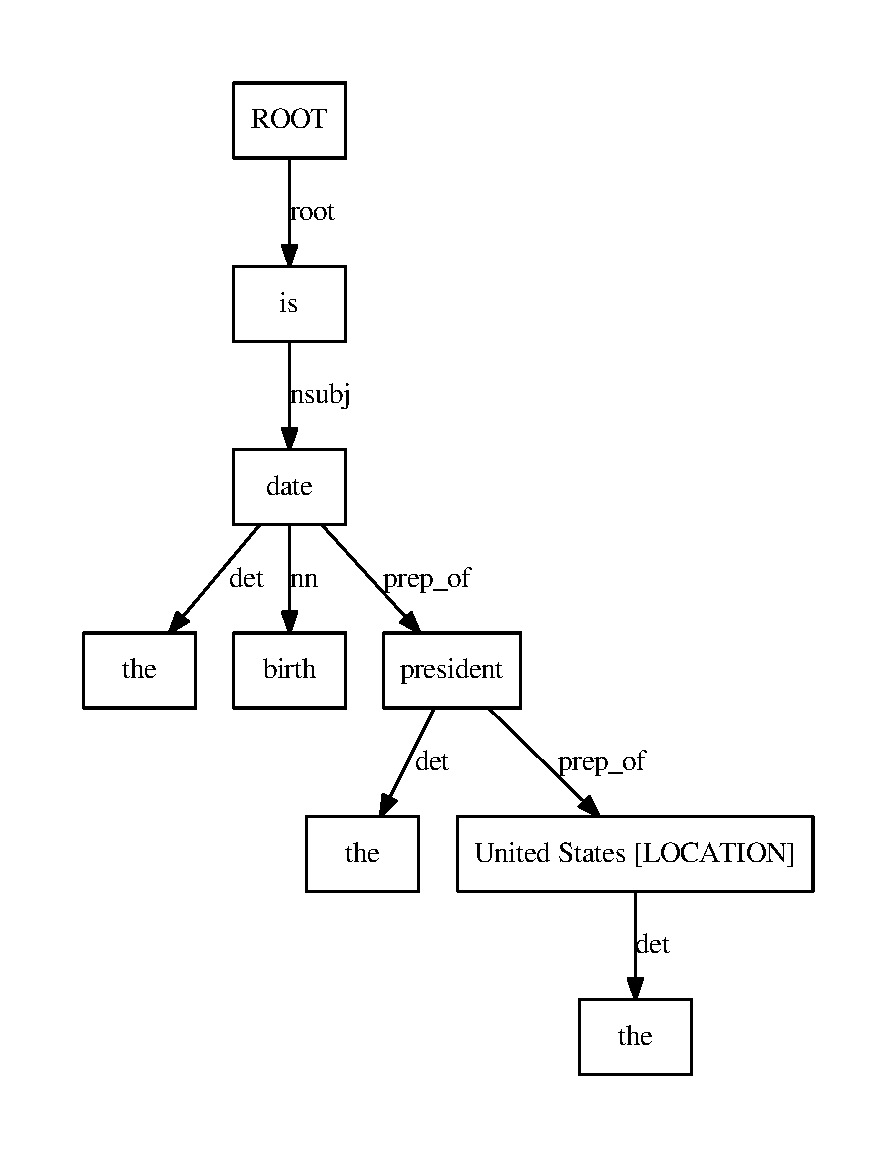
\includegraphics[scale=0.6]{../examples_NLP_grammatical/tree2.pdf}
\end{figure}

%########################################################################################%

\subsection{Grammatical dependencies analysis}

The grammatical tree is simplified by applying one of the following rules to each edge:
\begin{itemize}
 \item remove the edge and its endpoint node. For instance, a \textit{dep} relation, such as \textit{the} in our example, is often removed.
 \item merge the two nodes of the edge. Merge operations try to gather words of a same expression (e.g. phrasal verbs) that have not been merged during preprocessing.
 \item tag the edge with a ``triple production rule''.
\end{itemize}

The third operation is the most important. Dependencies relations are replaced by a restricted set of tags that will enable us to product a triples tree thereafter.

On our example, the edge:
\[\texttt{birth}\xrightarrow{\texttt{nn}}\texttt{date}\]

is merged into a single node : \textit{birth date}.

One of the triples production rules tag is : 

\[\texttt{is}\xrightarrow{\texttt{t1}}\texttt{birth date}\]

The simplified tree of our example is illustrated on figure \ref{tree_three}.

\begin{figure}
  \centering
  \caption{Dependency tree simplified}
  \label{tree_three}
    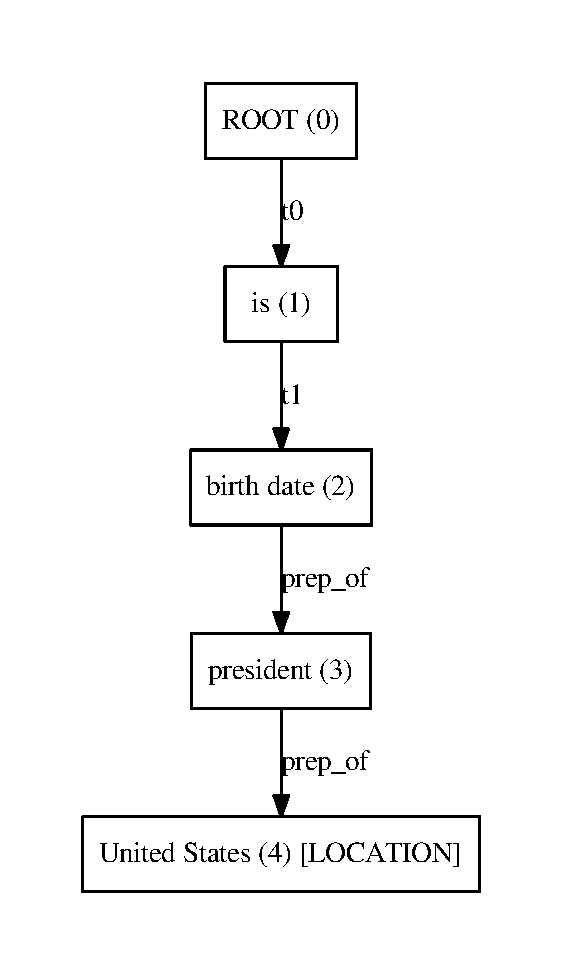
\includegraphics[scale=0.6]{../examples_NLP_grammatical/tree3.pdf}
\end{figure}

%########################################################################################%

\subsection{Triples production}

The triples production is the final step. It outputs the triples tree.

First, we assign a number to each remaining node. The root of the tree has always number \textit{0}. We have directly print these numbers on figure \ref{tree_three}.

Then, we associate to each subtree of root's number \textit{x} an unknown denoted \textit{?x} that identifies the information the subtree refers to. On our example, the subtree of root \textit{president} (number \textit{3}) represents the name of the president of the United States. This unknown is denoted \textit{?3}.

Unknowns are linked together into triples thanks to the triples production rules tagged previously. For instance, an  edge tagged \textbf{t2}:

\[\texttt{a}\xrightarrow{\texttt{t2}}\texttt{b}\]

products the triples \hl{(?a,a,?b)}, or \hl{(?a,a,b)} if b is a leaf (a and b are replaced by the words of the node they refer to).

The tag \textbf{t1} directly linked two unknowns \hl{?a = ?b}, instead of producing a triple.

The tag \textbf{t0} products nothing.

We obtain the following result on our example:

\begin{center}
 ?1 = ?2 ~\\
 (?2 , birth date of , ?3) ~\\
 (?3 , president of , United States)
\end{center}

Then, we link \textit{?0} to \textit{?1}, depending on the question word of the question. Here we have (question word \textit{What}):
\begin{center}
 (?1,definition,?0)
\end{center}

The four previous rules are simplified in a set a triples:

\begin{center}
 (?1,definition,?0) ~\\
 (?1 , birth date of , ?3) ~\\
 (?3 , president of , United States)
\end{center}

Find an answer to the question is equivalent to build a model of the conjunctive formula: \textbf{(?1 , definition , ?0)$\wedge$(?1 , birth date of , ?3)$\wedge$(?3 , president of , United States)} and outputs the value of \textit{?0}.

The triples tree is obtained by replacing each unknown \textit{?x} by a triple containing \textit{?x} \textit{and not} \textit{?0}. The final result, taken from the PPP website, is printed on figure \ref{tree_four}. Figure \ref{triple_tree} contains the formal representation of the triples tree of our example.

\begin{figure}[!h]
  \centering
  \caption{Triples tree}
  \label{tree_four}
    
\includegraphics[scale=0.5]{../examples_NLP_grammatical/final_result.png}
\end{figure}

Backend modules (such as Wikidata module) will have to fill intermediate unknowns : \hl{((August 4 1961,birth date of, (Barack Obama, president of, United States)), definition, ?)} and finally provide the final answer that replaced \textit{?} (for example: a description of the August 4 1961 date).


%########################################################################################%

\subsection{Future work}

\subsubsection{Grammatical rules analysis}

Our analysis of grammatical rules, in order to product triples, is very basic. Currently, we only have about 5 rules. Although it is good enough to handle a lot of questions, we are not able to process conjunctions for example (e.g. \textit{``Who wrote "Lucy in the Sky with Diamonds" and "Let It Be"?''}).

\subsubsection{Preprocessing merging}

There remains nodes which should stay together but are not merged by our module, for instance \emph{prime minister} or \emph{state of the art}. Recognizing such words is called \emph{Multiword Expressions Processing}. This task is a whole part of Natural Language Processing theory. 

We have several tracks to improve merging. Existing algorithms or softwares need to be tested. We could also use multiword expressions dictionaries.

\subsubsection{Question type analysis}

The current algorithm attaches great importance to the type of the input question. Sentences starting by a question word (Who, Where, How ...) are better processed than Yes/No questions for instance.

\subsubsection{Triples tree improvement}

The triples tree will be improved to take into account new types of nodes, adapted to databases queries. For example, a node could be tagged ``FIRST'' to pick the first occurrence of a list of answers (e.g. \hl{FIRST(?,presidents of, United States)}).


\subsection{Machine Learning \--- Reformulation}

\subsubsection{Aim}

\begin{frame}
\frametitle{Aim}
Asked questions are transformed in trees. But how to ensure the trees are adapted to our modules?
\pause
This is a translation module!!!! % TODO too many exclamation points

Changing the form, not the content.
\end{frame}

\subsubsection{Operation}
\begin{frame}
\frametitle{Operation}
Our tree is projected in a $\mathbb{R}$-vs: space of vectors.

\begin{defi}
The dictionary associates a vector triple to a word.

We wrote $(m.s,m.p,m.o)$ the triple of the word $m$. % TODO: what does it mean?
\end{defi}

\end{frame}

\begin{frame}
\frametitle{Projection}
\begin{tikzpicture}[x=2.5cm]
\node (s) at (1,0) {s};
\node (p) at (3,0) {p};
\node (r) at (2,1) {r};
\node (a) at (2,2) {a=compact(s,r,p)};
\node (b) at (4,2) {b};
\node (l) at (3,3) {l};
\node (h) at (3,4) {h=compact(a,l,b)};

\draw (s)--(a)--(p);
\draw (r)--(a);
\draw (a)--(h)--(b);
\draw (l)--(h);
\end{tikzpicture}
\end{frame}

\subsubsection{Build the request}

\begin{frame}
\frametitle{From vector to tree}
\begin{algorithm}[H]
\DontPrintSemicolon  % Some LaTeX compilers require you to use \dontprintsemicolon instead
\KwIn{$\delta>0$ et $a\in A$}
\KwOut{request tree}
$(s,p,o) \gets \text{uncompact}(a)$\;
Find m s.t. $\N{m.s-s}<\delta$ is minimal \;
\lIf{m exists}{$s \gets m.s$}
\lElse{$s \gets C(\delta,s)$} 
Find m s.t. $\N{m.o-o}<\delta$ is minimal \;
\lIf{m exists}{$o \gets m.o$}
\lElse{$o \gets C(\delta,o)$} 
$p \gets \text{argmin}_m.r (\N{m.r-m.p})$\;
\Return{$(s,r,o)$}\;
\caption{ From vector to tree }
\end{algorithm}

\end{frame}

\subsubsection{Learn}

\begin{frame}
\frametitle{Training}
Semantic distance.

Use relation graph ``instance of'' from Wikidata.
\end{frame} 


\section{Machine Learning: Window approach}

The goal of this module is to make an alternative to the grammatical approach, to product triples from English sentences.

We used machine learning algorithms in order to produce triples from scratch, without any grammatical library like \Stanford.


Motivations come from three points:
\begin{itemize}
\item Because triples are linked to the semantic of the sentence, and not directly from the grammar, we could expect that avoid grammatical tools can be a good idea.
\item It has been shown that a machine learning approach can produce, for a large panel of different NLP problems, very good solutions, closed to \textit{state of the art} algorithms \cite{collobert}.
\item Grammatical approaches fail on keyword sentences, like "Barack Obama birth date" because this kind of sentences does not respect the syntax of English.
\end{itemize}

This work is mainly based on the paper "Natural Language Processing (almost) from Scratch" \cite{collobert}.

Due to the restricted amount of time, we emphasis on keywords questions (keywords questions can't be analysis with grammatical tools) and we limit ourself to a restricted version of the data model:
\begin{itemize}
\item Only one level of depth: for example the sentence "What is the birth date of the president of the United States?" will be converted to the triple: \hl{(president of the United States, birth date, ?)}. 
\item We do not support \textit{types}, and connectors like \textit{first}, \textit{sort}...
\end{itemize}
We used a look-up table and a window approach neural network as explain below. The complete package\footnote{\url{https://github.com/ProjetPP/PPP-NLP-ML-standalone/}} was written in Python 3. We use the scikit-learn library, numpy and nltk as external tool.

Our algorithm can be described with three components: the look up table, the window approach, and the classifier.

\subsubsection{Look-up table}

The look-up table is a dictionary that associates to each word $w$ a vector $V_w \in \mathbb{R}^n$, where n is the number of parameters used to encode a word (we used $n=25$).
If two English words $w_1$ and $w_2$ are synonymous, then $||w_1-w_2||_2$ is small.

The construction of the look-up table is described in \cite{collobert} and used unsupervised machine learning techniques.
We used the pre-computed look-up table found here: \url{http://metaoptimize.com/projects/wordreprs/}

We also add one parameter to know if the word starts with a capitalize character or not. Finally, words are embedded in vectors of dimension 26. 

\subsubsection{Window approach}

We used a window (as explain in \cite{collobert}) that focuses on one word to classify. For example, if the sentence is "What is the birth date of the president of France?", and the word to classify is "date", for a window size of 7, the window is: "is the birth \textbf{date} of the president".


We used this window because classifier algorithms usually work with a fixed number of input parameters. 

The window size is a meta parameter to choose. This window has to be large enough that we can decide in the context of the window in which category a word is. We used a window of size 9.

\subsubsection{The classifier}

If the question is "What is the birth date of the president of France?", and the focus of the window approach is on the word \textbf{date}, then the goal is to classify the word \textbf{date} into one of these four categories: \textit{subject}, \textit{predicate}, \textit{object}, \textit{to forget}.

The classification of each word of the sentence into these four categories finally give us the desired triple.

The principle of the complete algorithm can be summarize in the figure ~\ref{sandalone:model}.

\begin{figure}[!ht]
  \centering
  \caption{The architecture of the algorithm, as described in \cite{collobert}}
  \label{sandalone:model}
    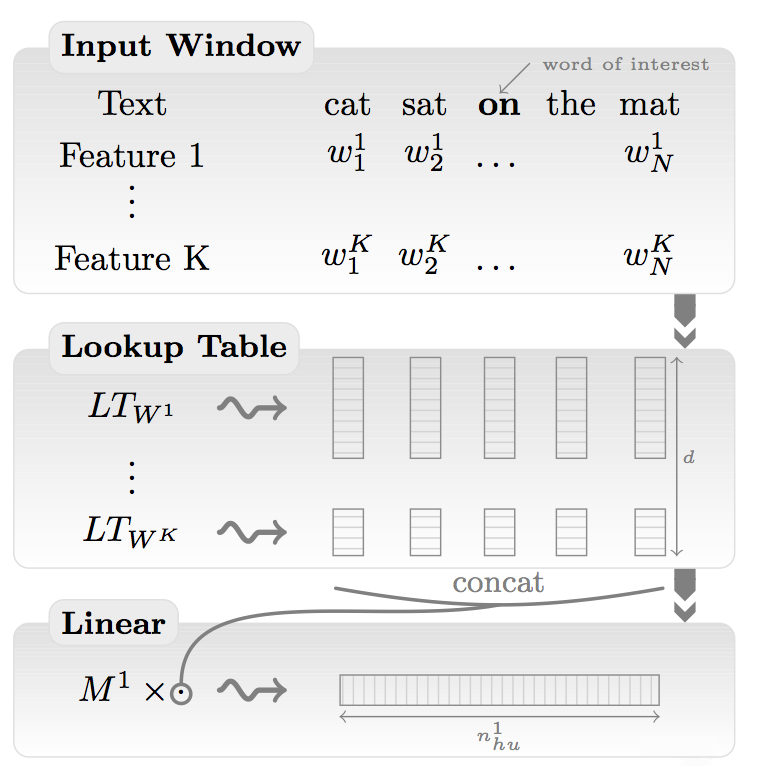
\includegraphics[scale=0.5]{../NLP-standalone-images/model.png}
\end{figure}

Because we have a small data set of annotated questions (see below), we used a linear model: a linear model has the advantage to have few parameters.
For example with a window approach of size 9 and words embedded in vectors of dimension 26,  this gives us $26\times 9\times 4 = 936$ parameters to learn.

In a first time we implemented our own linear classifier, but to improve the execution time, we finally used the \textit{LDA} classifier from the library scikit-learn. Few seconds of computation are now needed to train successfully the model.

\subsection{Data set}

Because we used supervised algorithms, we need a data set of annotated questions, in order to learn our model.
This data set was mostly built manually, because we did not find on the internet a data set that directly answering the problem of triple extraction.
Build this data set is a fastidious work. Currently our data set is composed of 300 questions.
We also wrote a script that generate keywords questions. This script gives us 500 keywords questions and make the module specialized on keywords questions.

We now denote $\mathcal{D}_{GC}$ (for \textit{Data set Grammatically Correct}) the data set of grammatically correct questions, $\mathcal{D}_{kw}$ for the data set of generated keywords questions and $\mathcal{D}_A = \mathcal{D}_{GC} \cup  \mathcal{D}_{KW}$ the complete data set.

\subsection{Results}

In this basic configuration, we can measure the accuracy of our algorithm, defined as the ratio of correctly classified words, for a specified data set.

Our methodology is the following: for a specified data set $\mathcal{D} \in \{\mathcal{D}_A, \mathcal{D}_{GC}, \mathcal{D}_{KW}\}$ we split $\mathcal{D}$ in two parts: the training set and the test set (90% of the data is for the training set and 10% for the testing set). We learn our classifier with the training set and then evaluate it on the test set.

\textbf{Remark}: to compute the accuracy of one variant of our algorithm we split the data set into testing and training set randomly, and we restart an experience 50 times. This make us sure of the precision of the estimated accuracy.

\begin{center}
\begin{tabular}{|l|c|r|}
  \hline
  Data set &  Testing accuracy  & Training accuracy \\
  \hline
  $\mathcal{D}_{GC}$ &  $75\%$& $81\%$  \\
  $\mathcal{D}_{KW}$ & $98\%$ & $98.3\%$ \\
  $\mathcal{D}_{A}$    & $83\%$ & $86\%$ \\
  \hline
\end{tabular}
\end{center}

We can conclude that this version of the algorithm is excellent for keyword questions, and not really good for grammatically correct questions.

\subsubsection{Bias vs Variance test}

We can plot the \textit{Bias versus Variance} curves:

\begin{figure}[!ht]
  \centering
  \caption{Bias vs Variance curve for the data set  $\mathcal{D}_{GC}$}
  \label{sandalone:bias_vs_variance_1}
    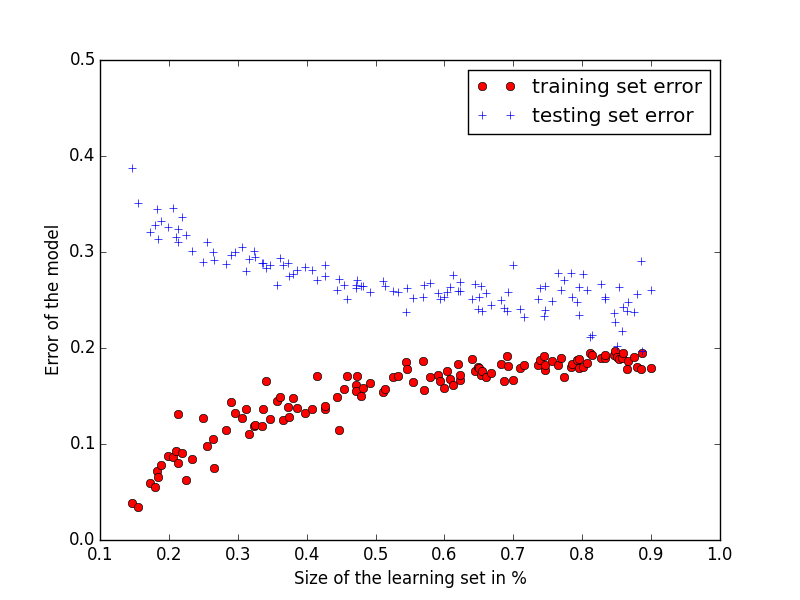
\includegraphics[scale=0.5]{../NLP-standalone-images/BiasVsVarianceD_GC.png}
\end{figure}

\begin{figure}[!ht]
  \centering
  \caption{Bias vs Variance curve for the data set  $\mathcal{D}_{KW}$}
  \label{sandalone:bias_vs_variance_2}
    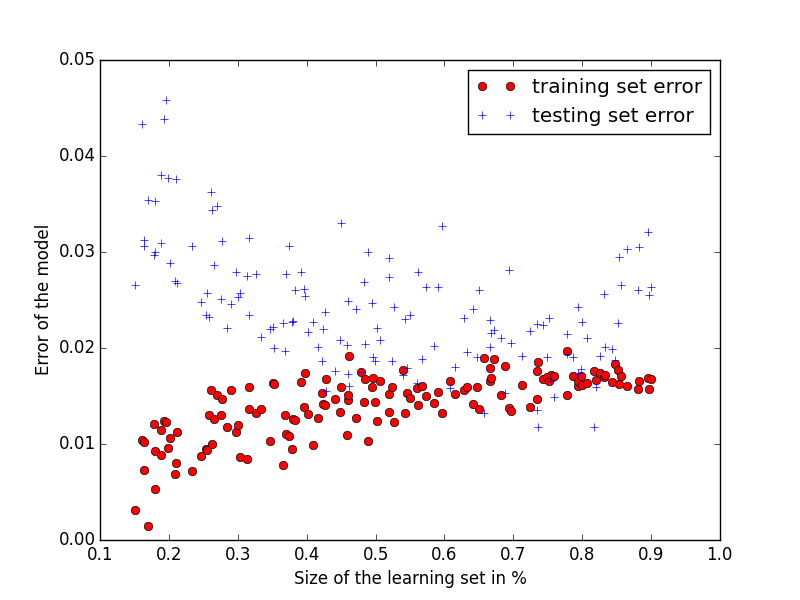
\includegraphics[scale=0.5]{../NLP-standalone-images/BiasVsVarianceD_KW.png}
\end{figure}

\begin{figure}[!ht]
  \centering
  \caption{Bias vs Variance curve for the data set  $\mathcal{D}_{A}$ }
  \label{sandalone:bias_vs_variance_3}
    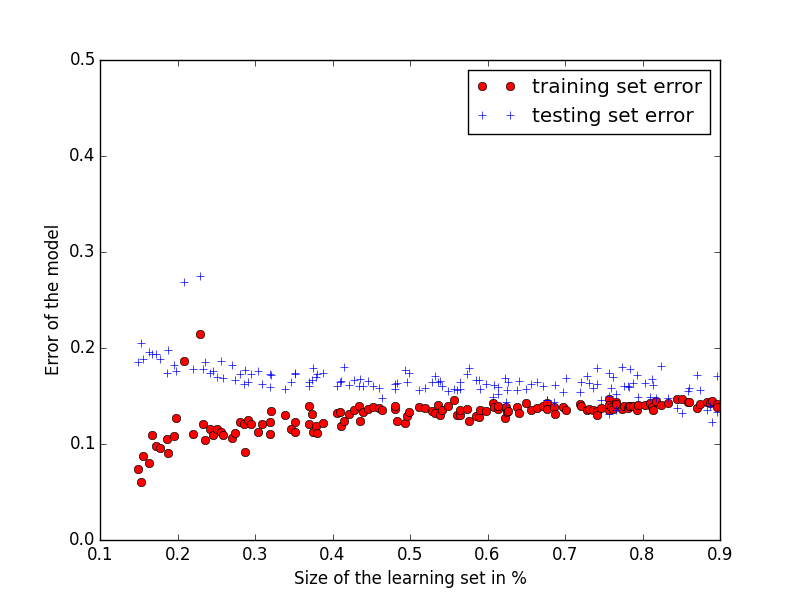
\includegraphics[scale=0.5]{../NLP-standalone-images/BiasVsVarianceD_A.png}
\end{figure}

These curves show us that there is a small gap between the two performances curves for the data set $\mathcal{D}_{GC}$: the data set of grammatically correct questions is too small to learn correctly the model.

However, when we add the keyword questions, the gap disappears: the model is learned correctly and the performances are good.

\subsection{Improvements of the algorithm}

\subsubsection{POS TAG features}

In order to help the classifier, we added POS TAG features: each word of the sentence is tagged with a grammatical tag (VERB, NOUN, PRON, ADJ, ...)

We use the NLTK pos tagger to do that. With such a tag, a word is encoded as a vector of dimension $26+11 = 37$.

This new feature helps improve the accuracy of the algorithm of few percents:

\begin{center}
\begin{tabular}{|l|c|r|}
  \hline
  Data set & Testing accuracy  without POS TAG & Testing accuracy  with POS TAG \\
  \hline
  $\mathcal{D}_{GC}$ &  $75\%$& $77.2\%$  \\
  $\mathcal{D}_{KW}$ & $98\%$ & $98.9\%$ \\
  $\mathcal{D}_{A}$    & $83\%$ & $86\%$ \\
  \hline
\end{tabular}
\end{center}


\subsection{Conclusion}

The initial goal was to make a concurrent of the grammatical approach to transform English questions into the data model. Due to the limited amount of time, we did not succeed to improve sufficiently the accuracy of the classifier to make this approach as good as the grammatical approach.

We decided then to focus on keywords questions, which are very important for a framework of question answering. For this task, whith a good data set of annotated keywords questions, this algorithm is really efficient.



\section{Back-end}

\Wikidata module is our main proof of concept module which aims to demonstrate the ability of our framework to allow the easy creation of huge modules able to answer to thousand of questions. This module tries to answer to general knowledge using the data stored in \href{http://www.wikidata.org}{\Wikidata}.

\Wikidata is a free knowledge base hosted by the \Wikimedia as a sister project of \Wikipedia. It aims to build a free, collaborative, multilingual structured database of general knowledge (for more information see \cite{42240}). It provides a very good set of API that allows to consume and query \Wikidata content easily. \Wikidata is built upon elements (called items) that are about a given subject. Each item has a label, a description and some aliases to describe it and statements that provides data about this subject.

The \Wikidata module has been written in PHP in order to rely on good libraries that allow to easily interact with the \Wikidata API. Some contributions to these libraries have been done to make them fit better with the module use case. This module works in tree steps:
\begin{enumerate}
    \item It maps \texttt{resource} nodes of the question tree into \Wikidata content: the subjects of \texttt{triple} nodes are mapped to \Wikidata items, predicates to \Wikidata properties and objects to the type of value that is the range of the \Wikidata property of the predicate. If more than one match are possible, a tree per possible match is output.
    \item It performs queries against \Wikidata content using the previously done mapping to reduce as much as possible trees. When we have a \texttt{triple} node where the object is missing the module gets the \Wikidata item of the subject, looks for values for the predicate property and replace the \texttt{triple} node with a \texttt{resource} node for each value of the triple (and so builds as many trees as there are values). When there is a \texttt{triple} node with a missing subject the module uses the \href{http://wdq.wmflabs.org}{WikidataQuery} tool API with \href{https://github.com/ProjetPP/WikidataQueryApi}{a standalone wrapper} built for the project that returns all items with a given statement.
    \item It adds clean text representation of \texttt{resource} nodes added by the previous phase.
\end{enumerate}

The global architecture of the module has been quickly studied by one of the \Wikidata developers that found it fairly good.


\subsection{CAS}
\begin{frame}[fragile]
    \frametitle{Computer Algebra System}
    Based on \alert{Sympy} (maths) and \alert{PLY} (parsers).
    
    \vfill    
    
    \onslide<2->{Two syntaxes:}
    \begin{itemize}
        \item<3-> Mathematica
        \item<4-> Intuitive syntax with permissive notations 
    \end{itemize}
\end{frame}

\subsection{Spell checker}


\begin{frame}[fragile]
    \frametitle{Spell Checker}
    Based on \alert{GNU Aspell}.

    \medbreak

    What are the langajes of Soth Afryka?

    $\rightarrow$

    What are the languages of South Africa?
\end{frame}


\section{Better than Wolfram?}
\begin{frame}[fragile]
    \frametitle{Nested question}

Who is the wife of the president of the United States?
    \begin{tabular}{ll}
        \alert{WolframAlpha} & Barack Obama\\
        \alert{Platypus} & Michelle Obama\\
    \end{tabular}

    \medbreak

    What are the birth dates of the daughters of the wife of the president of the United States?
    \begin{tabular}{ll}
        \alert{WolframAlpha} & Barack Obama\\
        \alert{Platypus} & Saturday, July 4, 1998 \& Sunday, June 10, 2001\\
    \end{tabular}
\end{frame}

\begin{frame}[fragile]
    \frametitle{Conjunction}

Who is an actor in Titanic and Inception?
    \begin{tabular}{ll}
        \alert{WolframAlpha} & all the actors of the two movies\\
        \alert{Platypus} & Leonardo DiCaprio\\
    \end{tabular}
\end{frame}

\section{Future work}

\begin{frame}[fragile]
    \frametitle{Better database}

    ``How fast is the TGV?''

    ``How wide is a tennis court?''

    Not answered by \alert{Wikidata}.

    \medbreak

    $\rightarrow$ Improve Wikidata?

    $\rightarrow$ Use another database?
\end{frame}

\begin{frame}[fragile]
    \frametitle{Better question parsing}

    ``What is the date of birth of Isaac Newton?''

    ``In which band does Bono sing?''

    Not parsed correctly.

    \medbreak

    $\rightarrow$ Train the Stanford CoreNLP library?

    $\rightarrow$ Improve the algorithm of the Grammatical module?

    $\rightarrow$ Better datasets for the ML modules?
\end{frame}

\begin{frame}[fragile]
    \frametitle{New modules}
    \begin{table}
    \Large
    \centering
    \begin{tabular}{ccc}
        \textcolor{mLightBrown}{cooking recipes} & \textcolor{mDarkBrown}{HAL} & \textcolor{mMediumBrown}{meteo} \\
        \multicolumn{3}{c}{\textcolor{mDarkTeal}{programming language interpreter}} \\
        \textcolor{mMediumBrown}{cinema} & \textcolor{mDarkTeal}{music} & \textcolor{mLightBrown}{literature}\\
        \textcolor{mDarkBrown}{OEIS} & \textcolor{mLightBrown}{translation} & \textcolor{mDarkTeal}{chemistry}\\
        \multicolumn{3}{c}{\textcolor{mMediumBrown}{sport statistics and predictions}} \\
    \end{tabular}
    \end{table}
\end{frame}

\begin{frame}[fragile]
    \frametitle{Some facts} % to update just before the presentation
    \alert{23 repositories}

    \begin{tabular}{lll}
        6 & PHP & Wikidata libraries and module\\
        12 & Python & Other modules, core, and libraries\\
        1 & C++ & ML-Reformulation\\
        1 & Shell & Deployment scripts\\
        1 & \LaTeX & This presentation and the report\\
        1 & Markdown & The specification\\
        1 & HTML/CSS/Javascript & The Web User Interface\\
        1 & HTML/CSS & The project's website\\
    \end{tabular}

    \alert{1982 commits} (without the ``integration'' repository, which has an automatic commit every 12h)

    \alert{26k lines} of code (13k in PHP, 10k in Python)
\end{frame}

\newlength{\logosize}
\setlength{\logosize}{12pt}
\begin{frame}[fragile]
    \frametitle{Stay tuned}
    \alert{\url{http://projetpp.github.io/}}

    \begin{tabular}{ll}
        
\includegraphics[width=\logosize]{Twitter_logo_blue.png} & \href{https://twitter.com/ProjetPP}{https://twitter.com/ProjetPP}\\
        
\includegraphics[width=\logosize]{GitHub-Mark-32px.png} &  \href{https://github.com/ProjetPP}{https://github.com/ProjetPP}\\
        
\includegraphics[width=\logosize]{ic_email_black_18dp.png} & \href{mailto:ppp@pony.ovh}{ppp@pony.ovh}\\
    \end{tabular}
\end{frame}


\begin{frame}
    \frametitle{Questions?}
    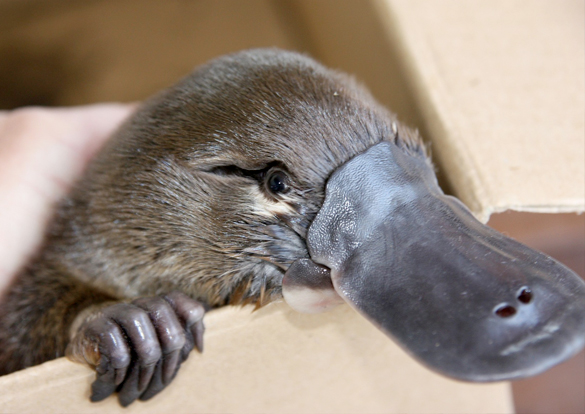
\includegraphics[width=\linewidth]{figures/platypusLg.jpg}
\end{frame}


\plain{Questions?}

\end{document}
